\chapter{Validation and Whole-System Review}
\label{chap:validation}

\section{Evidence status}

The verifier passes \val{94} validation checks and records the status
\path{ready_for_downstream_training}. The saved artifacts provide empirical
evidence for the data contract, split integrity, baseline comparisons, and
candidate holdout evaluation. This is a statement about the consistency and
readiness of the recorded workflow; it is not a statement that the current
candidate has passed the promotion gate or that the overall application is
production-ready.

The validation evidence should be read at three levels. At the data level,
the pipeline verifies row preservation, schema consistency, split separation,
and feature-order stability. At the modelling level, the saved comparisons
show how imbalance treatment and model family affect ranking and operating
metrics. At the application level, the packaged artefact can be loaded and
mapped to the scoring contract. The evidence is strongest for these recorded
local runs; it is weaker for long-running production concerns such as drift,
availability, access control, and performance under concurrent traffic.

\section{Reported validation results}

The accompanying project presentation and the repository artifacts report a
consistent validation story. At the data-processing level, the verifier passes
\val{94} checks with zero failures and produces the status
\path{ready_for_downstream_training}. The transaction--identity audit preserves
all \val{590,540} training transactions and all \val{506,691} test
transactions, while the chronological split produces \val{412,956} training,
\val{88,486} validation, and \val{89,098} holdout rows. The fraud rates in the
three windows remain close to the overall rate, which supports comparison
without replacing the time-ordered evaluation design.

At the model-selection level, CatBoost Balanced is the current candidate after
achieving the strongest recorded validation result in the model-family
comparison. Its validation PR-AUC is \val{0.5806} and validation ROC-AUC is
\val{0.9081}. These values support candidate selection, but they are not used
as a release claim by themselves. The holdout evaluation is deliberately
reported separately: holdout PR-AUC is \val{0.4266}, holdout ROC-AUC is
\val{0.8781}, precision is \val{0.3820}, recall is \val{0.5182}, and the
post-calibration Brier score is \val{0.0248}. The difference between validation
and holdout PR-AUC is the central reason the candidate remains unpromoted.

At the application level, the project reports that the backend can return a
calibrated fraud probability, a 0--100 risk score, a risk band, a decision, the
model version, and TreeSHAP attributions. The API supports both
\texttt{full\_feature} and \texttt{partial\_demo} scoring modes, while the
React review layer presents the score and explanation for analyst inspection.
This evidence demonstrates an integrated serving path; it does not establish
production latency, online feature parity, or autonomous decision safety.

\begin{table}[H]
\centering
\small
\rowcolors{2}{ReportGray!25}{white}
\caption{Consolidated validation and reported project results}
\label{tab:reported-validation-results}
\begin{tabularx}{\textwidth}{p{0.22\textwidth}p{0.25\textwidth}X}
\toprule
\textbf{Validation layer} & \textbf{Reported result} & \textbf{Interpretation}\\
\midrule
Data contract & \val{94} passed, \val{0} failed & Model-ready handover is structurally valid and traceable.\\
Chronological split & \val{412,956}/\val{88,486}/\val{89,098} rows & Time-ordered train, validation, and holdout windows are non-overlapping.\\
Candidate selection & Validation PR-AUC \val{0.5806}; ROC-AUC \val{0.9081} & CatBoost Balanced is the current challenger.\\
Holdout evaluation & PR-AUC \val{0.4266}; ROC-AUC \val{0.8781} & Later-period ranking quality falls below the promotion target.\\
Operating point & Precision \val{0.3820}; recall \val{0.5182}; Brier \val{0.0248} & The candidate provides a usable review trade-off, but requires policy and monitoring controls.\\
Promotion decision & \texttt{not\_promoted} & Holdout PR-AUC is below target \val{0.4582}; the serving default is unchanged.\\
\bottomrule
\end{tabularx}
\end{table}

The consolidated-results table provides one reading path across the system.
The first two rows establish that the data contract and chronological windows
are valid. The next rows show that CatBoost Balanced is strong during
validation but weaker on holdout, and that its operating threshold produces a
precision-recall trade-off suitable for review rather than blind automation.
The final row records the governance consequence: the candidate remains
unpromoted because the primary holdout ranking gate is not met.

\begin{figure}[H]
  \centering
  \begin{subfigure}[b]{0.48\textwidth}
    \centering
    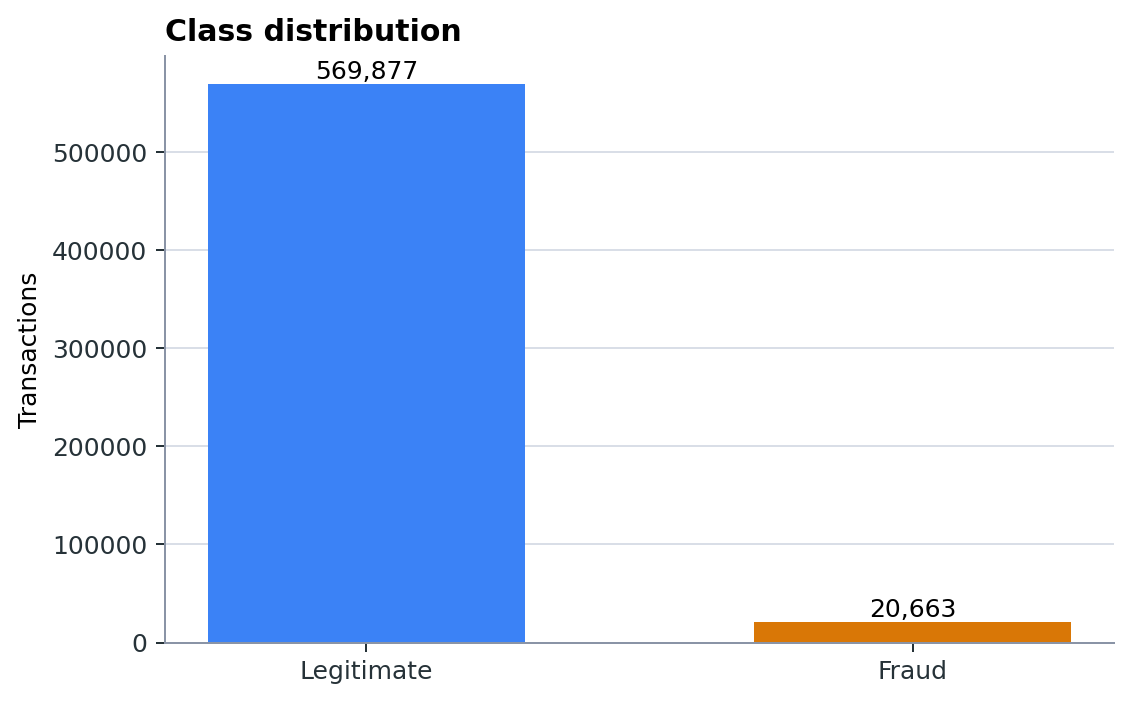
\includegraphics[width=\textwidth]{../../docs/figures/final_report/class-distribution.png}
    \caption{Class distribution.}
    \label{fig:final-class-distribution}
  \end{subfigure}
  \hfill
  \begin{subfigure}[b]{0.48\textwidth}
    \centering
    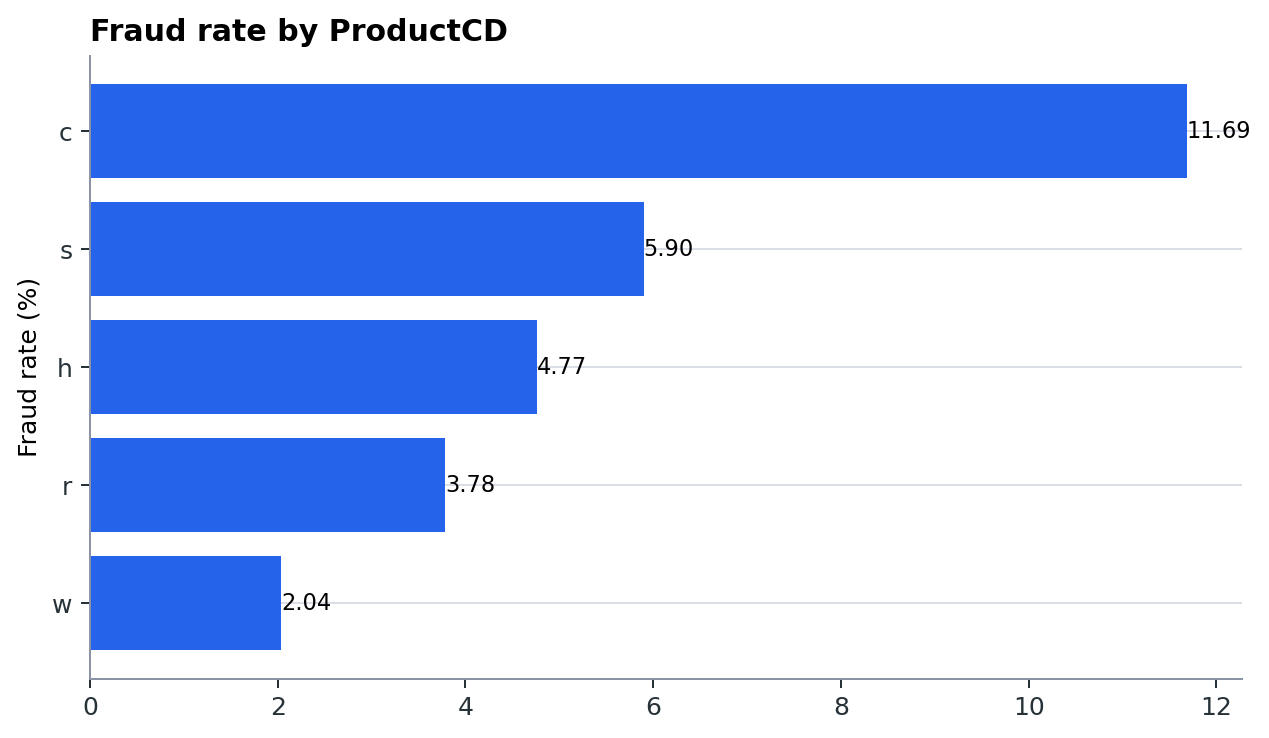
\includegraphics[width=\textwidth]{../../docs/figures/final_report/fraud-rate-by-product.png}
    \caption{Fraud rate by ProductCD.}
    \label{fig:final-fraud-product}
  \end{subfigure}
  \caption{Exploratory Data Analysis: Class distribution and fraud rate by ProductCD.}
  \label{fig:eda-overview-1}
\end{figure}

\begin{figure}[H]
  \centering
  \begin{subfigure}[b]{0.48\textwidth}
    \centering
    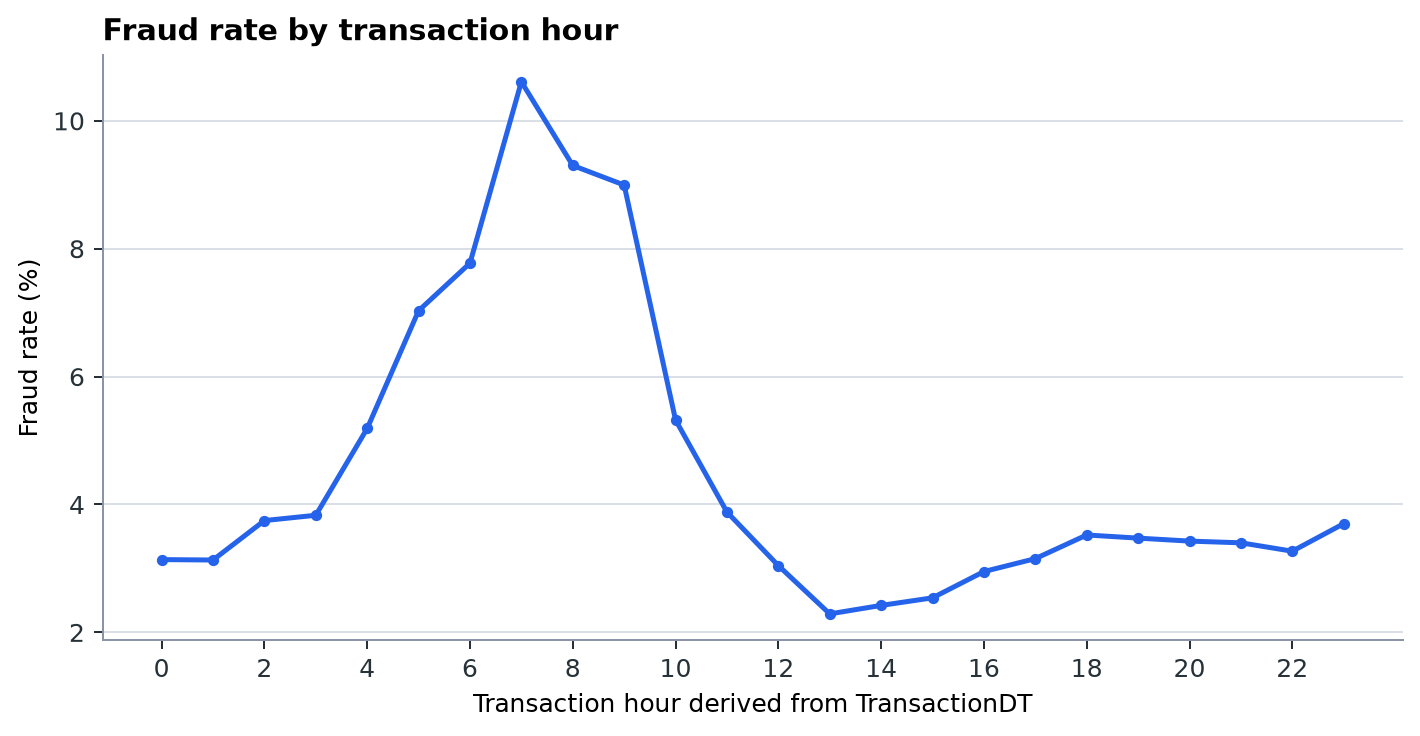
\includegraphics[width=\textwidth]{../../docs/figures/final_report/fraud-rate-by-transaction-hour.png}
    \caption{Fraud rate by transaction hour.}
    \label{fig:final-fraud-hour}
  \end{subfigure}
  \hfill
  \begin{subfigure}[b]{0.48\textwidth}
    \centering
    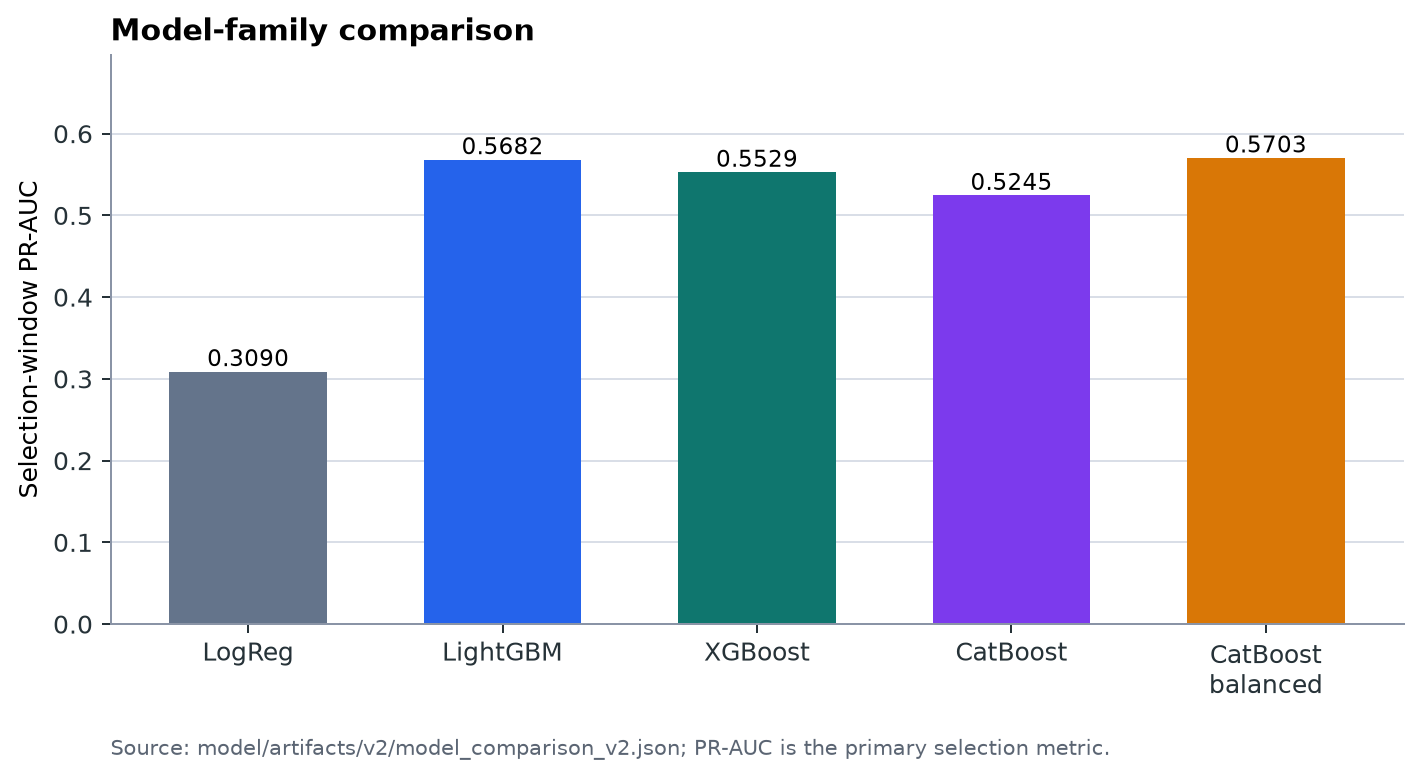
\includegraphics[width=\textwidth]{../../docs/figures/final_report/model-family-comparison.png}
    \caption{Model-family selection PR-AUC.}
    \label{fig:final-model-family}
  \end{subfigure}
  \caption{Temporal fraud association and model-family performance selection.}
  \label{fig:eda-and-model-family}
\end{figure}

\begin{figure}[H]
  \centering
  \begin{subfigure}[b]{0.48\textwidth}
    \centering
    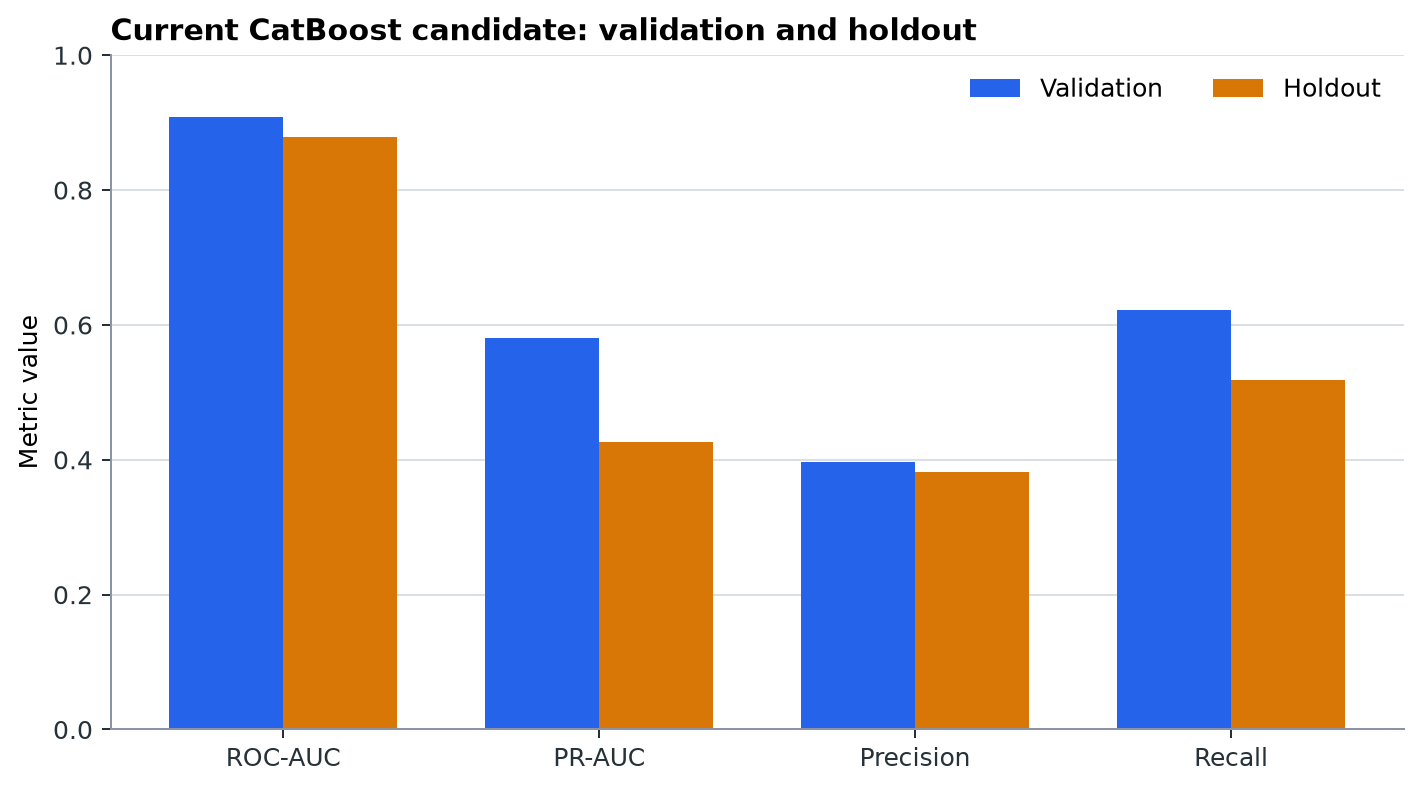
\includegraphics[width=\textwidth]{../../docs/figures/final_report/candidate-validation-holdout.png}
    \caption{Validation vs holdout metrics.}
    \label{fig:final-candidate-validation-holdout}
  \end{subfigure}
  \hfill
  \begin{subfigure}[b]{0.48\textwidth}
    \centering
    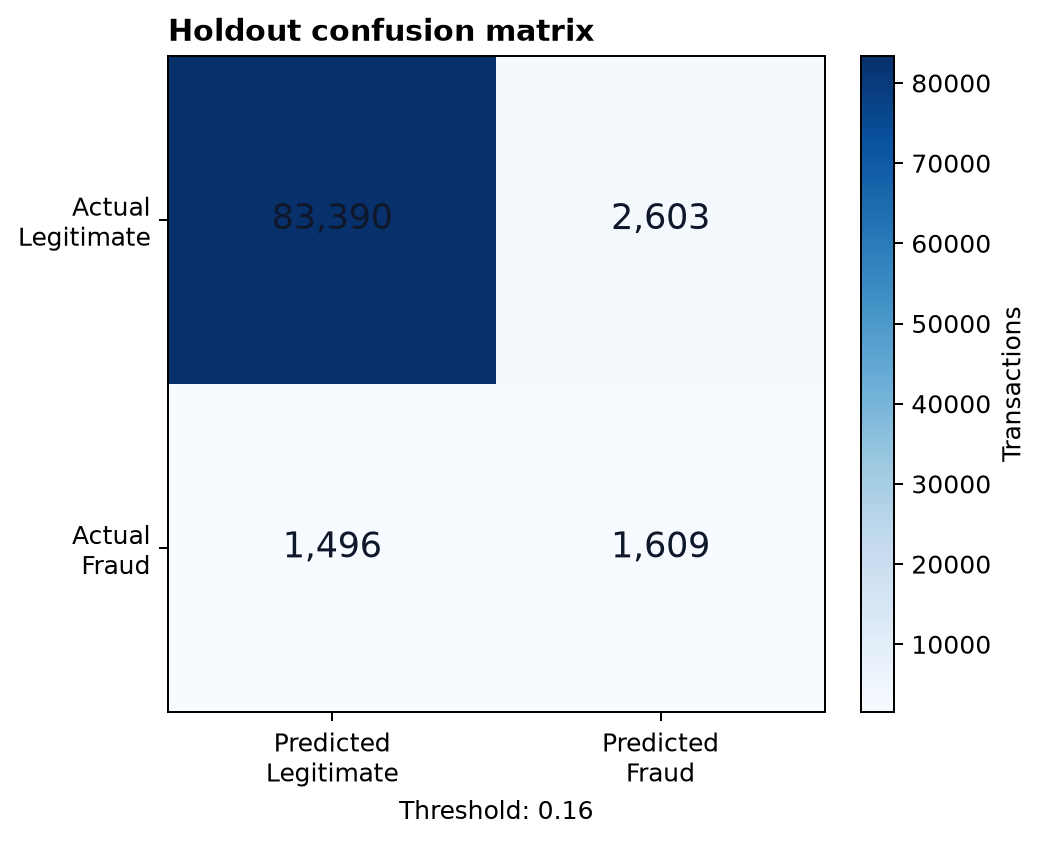
\includegraphics[width=\textwidth]{../../docs/figures/final_report/holdout-confusion-matrix.png}
    \caption{Holdout confusion matrix (0.16 threshold).}
    \label{fig:final-holdout-confusion}
  \end{subfigure}
  \caption{Candidate holdout evaluation: Metrics drop and operating confusion matrix.}
  \label{fig:model-holdout-eval}
\end{figure}

\begin{figure}[H]
  \centering
  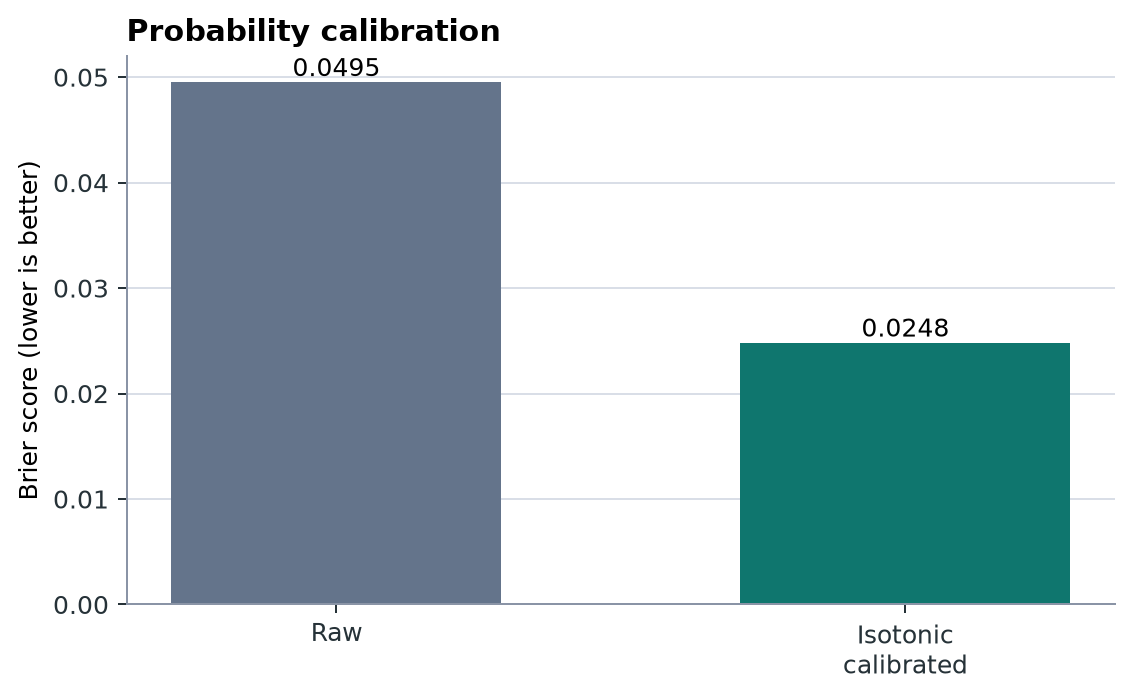
\includegraphics[width=0.55\textwidth]{../../docs/figures/final_report/calibration-brier.png}
  \caption{Probability calibration: Raw vs isotonic-calibrated Brier score on holdout.}
  \label{fig:final-calibration-brier}
\end{figure}


\section{Technical challenges and implemented solutions}

Table~\ref{tab:challenges-solutions} details the technical challenges, solutions, and repository evidence.

\begin{table}[H]
\centering
\small
\rowcolors{2}{ReportGray!25}{white}
\caption{Technical Challenges, Implemented Solutions, and Evidence}
\label{tab:challenges-solutions}
\begin{tabularx}{\textwidth}{>{\raggedright\arraybackslash}p{0.25\textwidth} X >{\raggedright\arraybackslash}p{0.25\textwidth}}
\toprule
\textbf{Challenge} & \textbf{Implemented solution} & \textbf{Evidence}\\
\midrule
Transaction--identity sparsity & Transaction-authoritative LEFT JOIN preserving 100\% transaction rows with missingness indicators & Preprocessing Join Audit Step\\
Missing values & Train-only median imputation for numeric; explicit \texttt{'missing'} category & Feature Contract Specification\\
Class imbalance & Evaluated \texttt{original}, \texttt{weighted} (weight 3.0), and \texttt{balanced} undersampled splits & Balanced Parquet Artifact\\
Temporal leakage & Chronological split on \texttt{TransactionDT} (\texttt{train} $\rightarrow$ \texttt{val} $\rightarrow$ \texttt{calib} $\rightarrow$ \texttt{holdout}) & Leakage-free Pipeline Stages\\
Schema \& feature order & Frozen canonical 68-feature vector and machine-checked schema hash gate & Verification Engine Gate\\
Verifier failure & Automated validation gate outputting \texttt{ready\_for\_downstream\_training} & Verification Report Artifact\\
Spark-to-pandas boundary & Spark handles distributed data preparation; Python fits single-node matrices & Model Execution Logs\\
Offline--online feature mismatch & Standardized backend feature loader mapping scoring request vector to schema & Backend Feature Loader\\
\bottomrule
\end{tabularx}
\end{table}

The challenges table connects each technical risk to an implemented control and
an evidence location. The controls are layered: row preservation protects the
join, train-only transformations protect against leakage, the frozen feature
vector protects compatibility, and the backend loader protects request-time
mapping. The table also shows where the controls stop, since offline--online
mismatch and the Spark-to-pandas boundary remain known limitations.

\section{Consolidated limitations}

The first limitation concerns reproducibility at scale: experiment tracking is local and the estimator stage uses single-node pandas-compatible matrices, so the workflow has a clear memory and operational ceiling. The second concerns policy alignment: backend risk bands are configured separately from offline threshold optimisation, which can cause the displayed decision policy and the evaluated operating point to diverge. The third concerns offline--online parity because a real-time feature store for historical aggregates has not been implemented; the API therefore cannot yet guarantee that every online aggregate is calculated in exactly the same way as its training counterpart. The fourth concerns operational controls, since the demonstration includes a fail-open heuristic and in-memory background jobs that could conceal model-loading failures or lose work after restart. The fifth concerns security and governance: authentication, role-based authorization, and durable audit logging are not complete, so the system should not be used to make unsupervised real-world decisions.

These limitations affect how the results should be used. The model metrics are
appropriate for comparing the recorded candidates and for demonstrating a
controlled validation procedure. They are not sufficient to estimate fraud
loss reduction, customer impact, or regulatory suitability in a live business
context. Before operational use, the project would need an online feature
parity test, a policy calibration study with real review capacity, security
testing, durable audit trails, drift monitoring, rollback procedures, and
repeated evaluation on later data. The explicit limitation statement is thus a
guardrail around interpretation, not a rejection of the current results.
